\def\mytitle{Advance Optimization Assignment}
\def\myauthor{A.Gowri Priya}
\def\contact{gowripriyaappayyagari@gmail.com}
\def\mymodule{Future Wireless Communication (FWC)}
\documentclass[10pt, a4paper]{article}
\usepackage[a4paper,outer=1.5cm,inner=1.5cm,top=1.75cm,bottom=1.5cm]{geometry}
\twocolumn
\usepackage{setspace}
\usepackage{graphicx}
\graphicspath{{./images/}}
\usepackage[colorlinks,linkcolor={black},citecolor={blue!80!black},urlcolor={blue!80!black}]{hyperref}
\usepackage[parfill]{parskip}
\usepackage{lmodern}
\usepackage{tikz}
	\usepackage{physics}
%\documentclass[tikz, border=2mm]{standalone}
\usepackage{karnaugh-map}
\usepackage{tabularx}
\usetikzlibrary{calc}
\usepackage{amsmath}
\usepackage{amssymb}
\renewcommand*\familydefault{\sfdefault}
\usepackage{watermark}
\usepackage{lipsum}
\usepackage{xcolor}
\usepackage{listings}
\usepackage{float}
\usepackage{titlesec}
\providecommand{\mtx}[1]{\mathbf{#1}}
\titlespacing{\subsection}{1pt}{\parskip}{3pt}
\titlespacing{\subsubsection}{0pt}{\parskip}{-\parskip}
\titlespacing{\paragraph}{0pt}{\parskip}{\parskip}

\newcommand{\myvec}[1]{\ensuremath{\begin{pmatrix}#1\end{pmatrix}}}
\let\vec\mathbf
\lstset{
frame=single, 
breaklines=true,
columns=fullflexible
}
\title{\mytitle}
\author{\myauthor\hspace{1em}\\\contact\\FWC22012\hspace{6.5em}IITH\hspace{0.5em}\mymodule\hspace{6em}ASSIGN-8}
\date{}
\begin{document}
	\maketitle
\section{Problem}
Find the point on the curve \begin{math}
x^2 =8y
\end{math} which is nearest to the point (2, 4)?
\section{Solution}
The given problem can be expressed as
\begin{align}
\min\norm{\vec{x}-\vec{P}}^2
\\
\text{s.t. }\vec{x}^T\vec{V}\vec{x} + \vec{u}^T\vec{x}  +d = 0
\end{align}
where
\begin{align}
\vec{V} &= \myvec{1 & 0\\0 & 0}
\\
\vec{u} &= -\myvec{0 \\ 8}
\\
d &= 0
\end{align}
\begin{align}
\min{(\vec{x}-\vec{P})}^T{(\vec{x}-\vec{P})}
\\
\text{s.t. }\vec{x}^T\vec{V}\vec{x} + \vec{u}^T\vec{x}  \le 0
\end{align}
The following code yields the minimum distance as 2.069 and the nearest point on the curve as
\begin{align}
\vec{Q} &= \myvec{4\\2}
\end{align}
\begin{lstlisting}
codes/opt/qp_cvx.py
\end{lstlisting}
\section{Construction}
\begin{figure}[h]
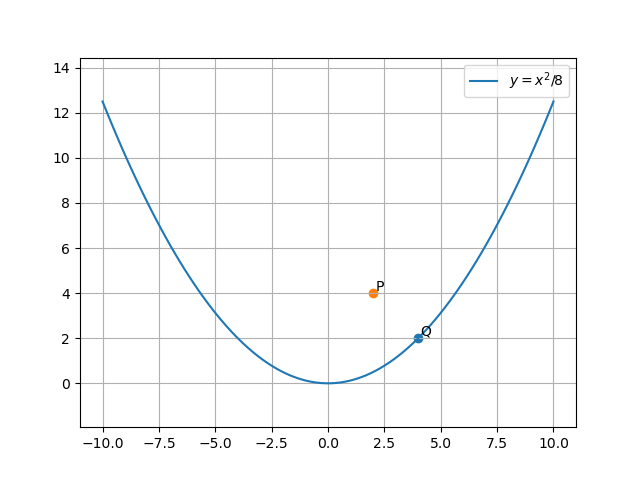
\includegraphics[scale=0.5]{aopp.png} 
\end{figure}
\framebox{
\url{https://github.com/gowripriya-2002/FWC/blob/main/Optimization/Advance/code/aop.py}}
\end{document}
